\documentclass{beamer}
\mode<presentation>{
  \usetheme{Warsaw}

  \definecolor{beamer@blendedred}{rgb}{0.7,0.1,0.1}
  \setbeamercolor{structure}{fg=beamer@blendedred}

  \setbeamercovered{invisible}
}

\usepackage[T2A]{fontenc}
\usepackage[utf8]{inputenc}
\usepackage[russian]{babel}
\usepackage{multimedia}
\logo{
\includegraphics[height=0.3cm]{valknut.png}}



\title{Почему ФП?}
\author{Максим Трескин\\ \texttt{maxim.treskin@gmail.com} \\ \texttt{@mtreskin}}
\date[2010.10.02]{2 октября, 2010}

\begin{document}

\begin{frame}
  \titlepage
\end{frame}




\begin{frame}
  \frametitle{Функциональное программирование}
  \begin{itemize}
  \item Сначала был матан: Алонзо Чёрч придумал $\lambda$-исчисления
    \pause
  \item Затем практика: Джон Маккарти открыл Lisp, содержащий реализацию $\lambda$-исчисления
  \end{itemize}
\end{frame}


\begin{frame}
  \frametitle{В чём соль?}
  \begin{itemize}
  \item Не изменяется состояние
    \pause
  \item Хвостовая рекурсия
    \pause
  \item Функции первого класса
    \pause
  \item Алгебраические типы и сопоставление шаблону
  \end{itemize}
\end{frame}

\begin{frame}
  \frametitle{Неизменяемое состояние}
  \begin{itemize}
  \item Сложно накосячить
    \pause
  \item Легко тестировать
    \pause
  \item Легко распределять
  \end{itemize}
\end{frame}


\begin{frame}[fragile]
  \frametitle{Хвостовая рекурсия}
  \begin{block}{}
\begin{verbatim}
State = {inc:integer = 0}

iterate(State) ->
    NewState = State{inc + 5}
    iterate(NewState)
\end{verbatim}
  \end{block}

\end{frame}


\begin{frame}
  \frametitle{Обычное выполнение рекурсии}
  \begin{itemize}
  \item Записали на стек адрес, куда надо вернуться
    \pause
  \item Вызвали функцию с начальными параметрами
    \pause
  \item Записали на стек адрес, куда надо вернуться
    \pause
  \item Вызвали функцию с новыми параметрами
    \pause
  \item Повторить до завершения памяти
    \begin{center}
      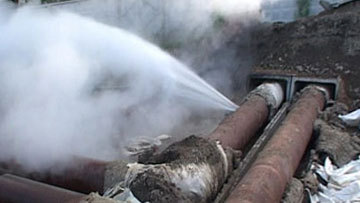
\includegraphics[height=4cm]{overflow.png}
    \end{center}

  \end{itemize}
\end{frame}

\begin{frame}
  \frametitle{Xzibit, прокачай нашу рекурсию}
  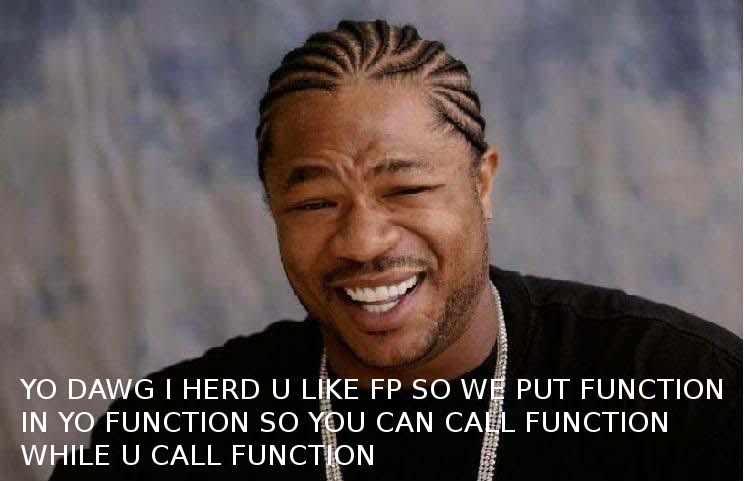
\includegraphics{xzibit-happy.png}
\end{frame}

\begin{frame}
  \frametitle{Xzibited выполнение рекурсии}
  Транслятор преобразует хвостовую рекурсию в итерацию!
  \pause
  \begin{itemize}
  \item Записали на стек адрес, куда надо вернуться
    \pause
  \item Вызвали функцию c начальными параметрами
    \pause
  \item Вызвали функцию c новыми параметрами
    \pause
  \item Вызвали функцию c новыми параметрами
    \pause
  \item Повторить до выключения питания
    \begin{center}
      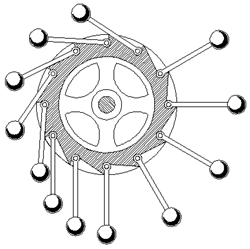
\includegraphics[height=4cm]{perpetuum.png}
    \end{center}
  \end{itemize}
\end{frame}

\begin{frame}
  \frametitle{Функции первого класса}
  \begin{itemize}
  \item Функции высшего порядка
    \pause
  \item Замыкания
  \end{itemize}
\end{frame}

\begin{frame}
  \frametitle{Функции высшего порядка}
  Можно присваивать функции переменным и передавать их в другие функции
  \begin{block}{}
    \texttt{{\color{blue}map} f [] = []}

    \texttt{{\color{blue}map} f (x:xs) = f x : map f xs}
    \pause

    \texttt{{\color{blue}add1} x = x + 1}
    \pause

    \texttt{{\color{blue}map} add1 [1,2,3]}

    \texttt{[2,3,4]}
  \end{block}
\end{frame}

\begin{frame}[fragile]
  \frametitle{Замыкания}
  \pause
  На vasya@pupkin:

  \begin{block}{}
    \texttt{M = 14,}

    \texttt{Fun = {\color{magenta}fun}(X) ->}

    \verb+        +\texttt{{\color{magenta}io:format}({\color{orange}``M = \~{}b, X = \~{}b\~{}n``}, [M, X])}

    \verb+      +\texttt{{\color{magenta}end},}

    \texttt{\{eye, {\color{blue}tolya@pipkin}\} ! Fun.}

  \end{block}
  \pause

  На tolya@pipkin:

  \begin{block}{}
    \texttt{Rcv = {\color{magenta}fun}() ->}

    \verb+        +\texttt{{\color{magenta}receive} M -> M(55) {\color{magenta}end}}

    \verb+      +\texttt{{\color{magenta}end},}

    \texttt{Pid = {\color{magenta}spawn}(Rcv)}

    \texttt{{\color{magenta}register}(eye, Pid).}

  \end{block}

  \pause

  \begin{block}{}
    \texttt{M = 14, X = 55}
  \end{block}




\end{frame}


\begin{frame}
  \frametitle{Алгебраические типы}
  \begin{center}
    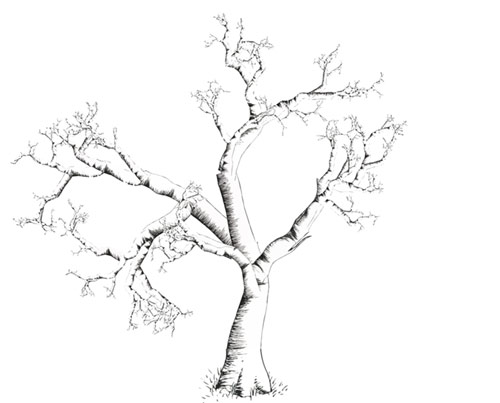
\includegraphics[height=6cm]{tree.png}
  \end{center}
\end{frame}

\begin{frame}[fragile]
  \frametitle{Алгебраические типы}
  \begin{block}{}
    \texttt{{\color{magenta}тип} {\color{blue}Живность} =}
      \pause

      \verb+    +\texttt{{\color{blue} Человек} Пол:{\color{magenta}bool}, ЦветВолос:{\color{magenta}color}}
      \pause

      \verb+  +\texttt{| {\color{blue}Червь} Длина:{\color{magenta}int}}
      \pause

      \verb+  +\texttt{| {\color{blue}Гусеница} Лапы:{\color{magenta}int}}
      \pause

      \verb+  +\texttt{| {\color{blue}Цикада} Громкость:{\color{magenta}int}}
      \pause

      \verb+  +\texttt{| {\color{blue}Мертвяк}}
  \end{block}
\end{frame}

\begin{frame}
  \frametitle{Сопоставление шаблону}
  \begin{center}
    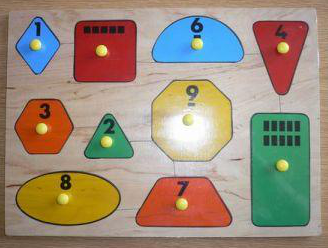
\includegraphics[height=6cm]{pm.png}
  \end{center}
\end{frame}

\begin{frame}[fragile]
  \frametitle{Сопоставление шаблону}
  \begin{block}{}
    \texttt{{\color{red}что\_делать} :: {\color{blue}Живность} -> {\color{blue}Action}}
    \pause

    \texttt{{\color{red}что\_делать}(Ж:{\color{blue}Живность}) ->}

    \verb+  +\texttt{{\color{magenta}сравним} Ж {\color{magenta}с}:}
    \pause

    \verb+    +\texttt{({\color{blue}Человек} Пол={\color{red}да}, ЦветВолос=\_) -> {\color{red}да};}
    \pause

    \verb+    +\texttt{({\color{blue}Цикада} Громкость=\$г) ->}

    \verb+        +\texttt{{\color{magenta}если} \$г > 100 -> {\color{red}убегать},}

    \verb+        +\texttt{{\color{magenta}иначе} -> {\color{red}слушать};}
    \pause

    \verb+    +\texttt{({\color{blue}Мертвяк}) -> {\color{red}сообщить\_куда\_надо};}
    \pause

    \verb+    +\texttt{(\_) -> {\color{red}созерцать}.}
  \end{block}
\end{frame}

\begin{frame}
  \frametitle{А также...}
  \begin{itemize}
  \item Ленивость
    \pause
  \item Карринг
    \pause
  \item Вывод типов
    \pause
  \item Просто хороший синтаксис
    \pause
  \item И ещё много чего хорошего
  \end{itemize}
\end{frame}

\begin{frame}
  \frametitle{Функциональные языки программирования}
  \begin{itemize}
  \item Erlang
    \pause
  \item SML, OCaml, F\#
    \pause
  \item Scala, Clojure
    \pause
  \item Haskell
  \end{itemize}
\end{frame}

\begin{frame}
  \frametitle{Ресурсы}
  \begin{itemize}
  \item http://fprog.ru
  \item http://erlanger.ru
  \item erlang-russian, scala-russian, clojure-russian на гуглогруппах
  \item Конференции на jabber.ru
  \end{itemize}
\end{frame}



\begin{frame}
  \frametitle{Вопросы?}
  \titlepage
\end{frame}




\end{document}
